\chapter{Desenvolvimento da Plataforma}

Para desenvolver a plataforma é necessário um projeto estrutural em conjunto com o projeto eletrônico da Placa de Circuito Impresso (PCI) que irá embarcar os componentes eletrônicos. 

\section{Projeto Estrutural}
Dentre as variações de modelo Barn-Door que foram abordadas na seção \ref{sec:modelosdemontagem}, optou-se pelo modelo de rosca curvada, que é mais simples e barato dentre as outras opções. A montagem de braço simples foi descartada pois ela requer que o motor tenha um feedback do ângulo da plataforma para regular sua correta velocidade, isso encarece o sistema tornado-o mais complexo. Ao contrário, a montagem de braço dupla não possui esse último problema, porém requer uma montagem mais elaborada e com mais componentes mecânicos, deixando a desejar no fator simplicidade. 

\subsection{Requisitos de Projeto}
Apesar da montagem curva ter suas vantagens, ela também apresenta características estruturais que requerem atenção durante o projeto; não só por problemas inerente da montagem curva, mas também por caracterizar problemas genéricos de qualquer montagem Barn-Door. Então, destacam-se abaixo os requisitos mais relevantes para este trabalho:

\begin{itemize}
	\item Mover a câmera com uma velocidade angular constante de $ 0,2507^{\circ}/min $. 
	\item Suportar pelo menos 2kg de peso total em rastreamento. 
	\item Ter peso máximo de 1kg sem a câmera.
	\item Possuir vibração -- em rastreamento e nos 3 eixos inerciais -- que não seja visível no sensor da câmera.
\end{itemize}

\subsection{Motor 28BYJ-48}
O motor selecionado foi o modelo 28BYJ-48 (Figura \ref{fig:28byj}), por ser de baixo custo e funcionar com tensão de alimentação 5V. A importância disso será abordada na próxima seção. O Motor possui 4 fases e $ 2048 $ passos em modo Full Step; o \textit{pull in} torque é de $ 29,43~mN.m $ \cite{man:stepperMotor}.

\begin{figure}[!htb]
	\centering
	\caption{Motor de Passo 28BYJ-48}
	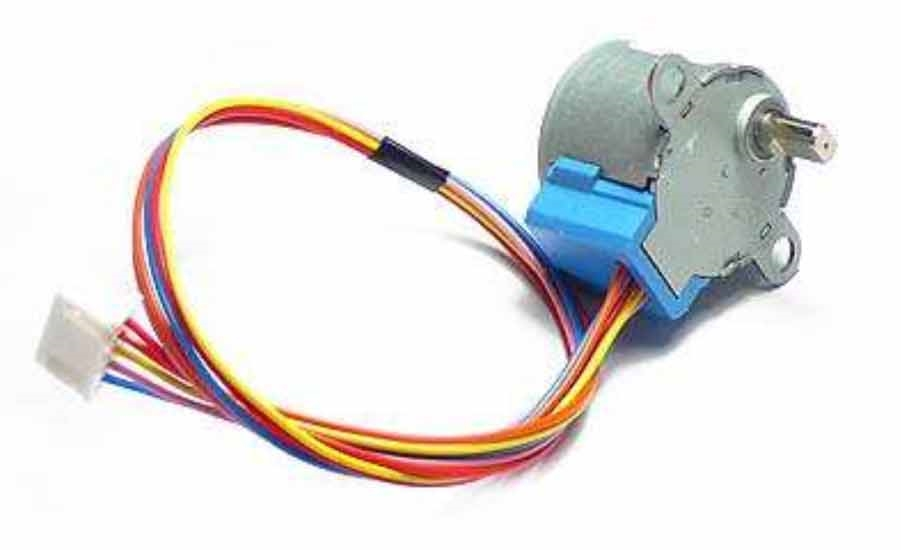
\includegraphics[width=0.7\linewidth]{figuras/desPlataforma/motordepasso}
	\label{fig:28byj}
	\fonte{\cite{man:stepperMotor}.}
\end{figure}


\subsection{Estrutura Principal}

A estrutura principal é a parte responsável por abrigar todos os componentes, fixar a câmera e também ser fixada no tripé do fotógrafo. Ela foi projetada com MDF 15mm pois é um material economicamente mais viável que metais, e consegue prover resistência ao sistema. O projeto das peças nomeadas de base superior e base inferior se conecta com uma dobradiça comum, e é demonstrado na Figura \ref{fig:renderMontagem} com a região interna em amostra.

\begin{figure}[!htb]
	\centering
	\caption{Encaixe das peças superior e inferior}
	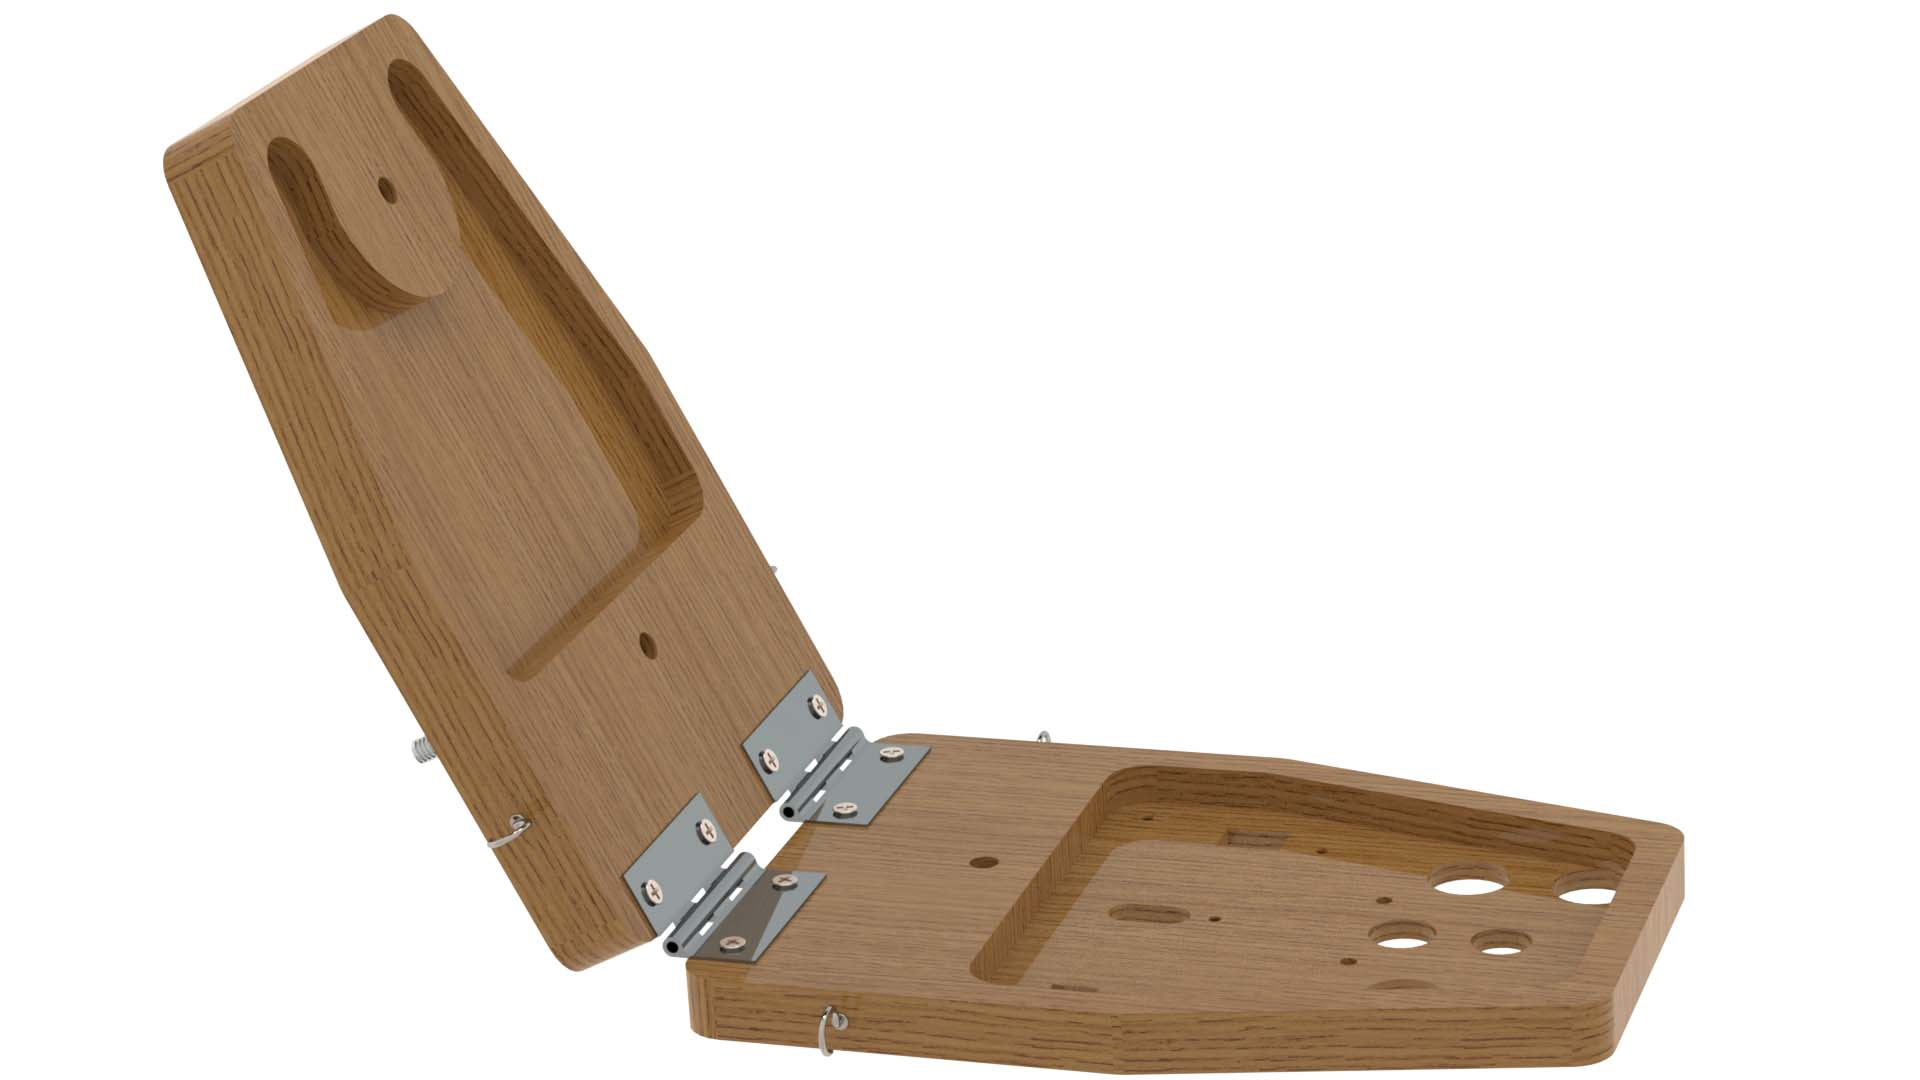
\includegraphics[width=.8\linewidth]{figuras/desPlataforma/renderMontagem}
	\label{fig:renderMontagem}
	\fonte{Autor.}
\end{figure}

É possível reparar que ambas as peças possuem um corte interno, que não é passante, e tem como função alocar todos os componentes. No entanto, esse tipo de corte é mais caro do que um passante fabricado à Laser, por exemplo, e por isso sugere-se que os componentes eletrônicos sejam simplificados em projetos futuros.

A base superior fixa a câmera, e a base inferior é fixada no tripé do fotógrafo. Essa fixação da base inferior é realizada usando um inserto roscado para madeira de 1/4" (Figura \ref{fig:insertoMadeira}), que fica instalada como demonstra a Figura \ref{fig:insertoMontagem}. A fixação da câmera na base superior é realizada usando um Ball-Head. No CAD, isso foi representado usando um modelo de Ball Head simplificado (Figura \ref{fig:renderMontagemCamera}), porém o sistema consegue suportar qualquer modelo, uma vez que a fixação desses componentes é feita por meio de uma rosca padrão de 3/8".

\begin{figure}[!htb]
	\centering
	\caption{Fixação no tripé: (a) Inserto e (b) Montagem}
	\captionsetup[subfigure]{justification=centering}
	\begin{subfigure}[b]{0.24\textwidth}
		\centering
		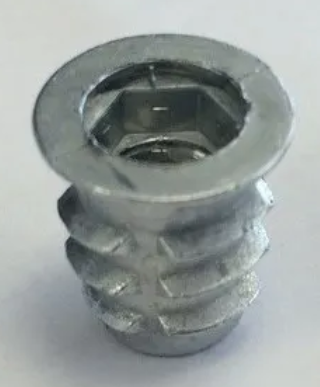
\includegraphics[width=\textwidth]{figuras/desPlataforma/insertoMadeira}
		\caption{}
		\label{fig:insertoMadeira}
	\end{subfigure}
	\hfill
	\begin{subfigure}[b]{0.74\textwidth}
		\centering
		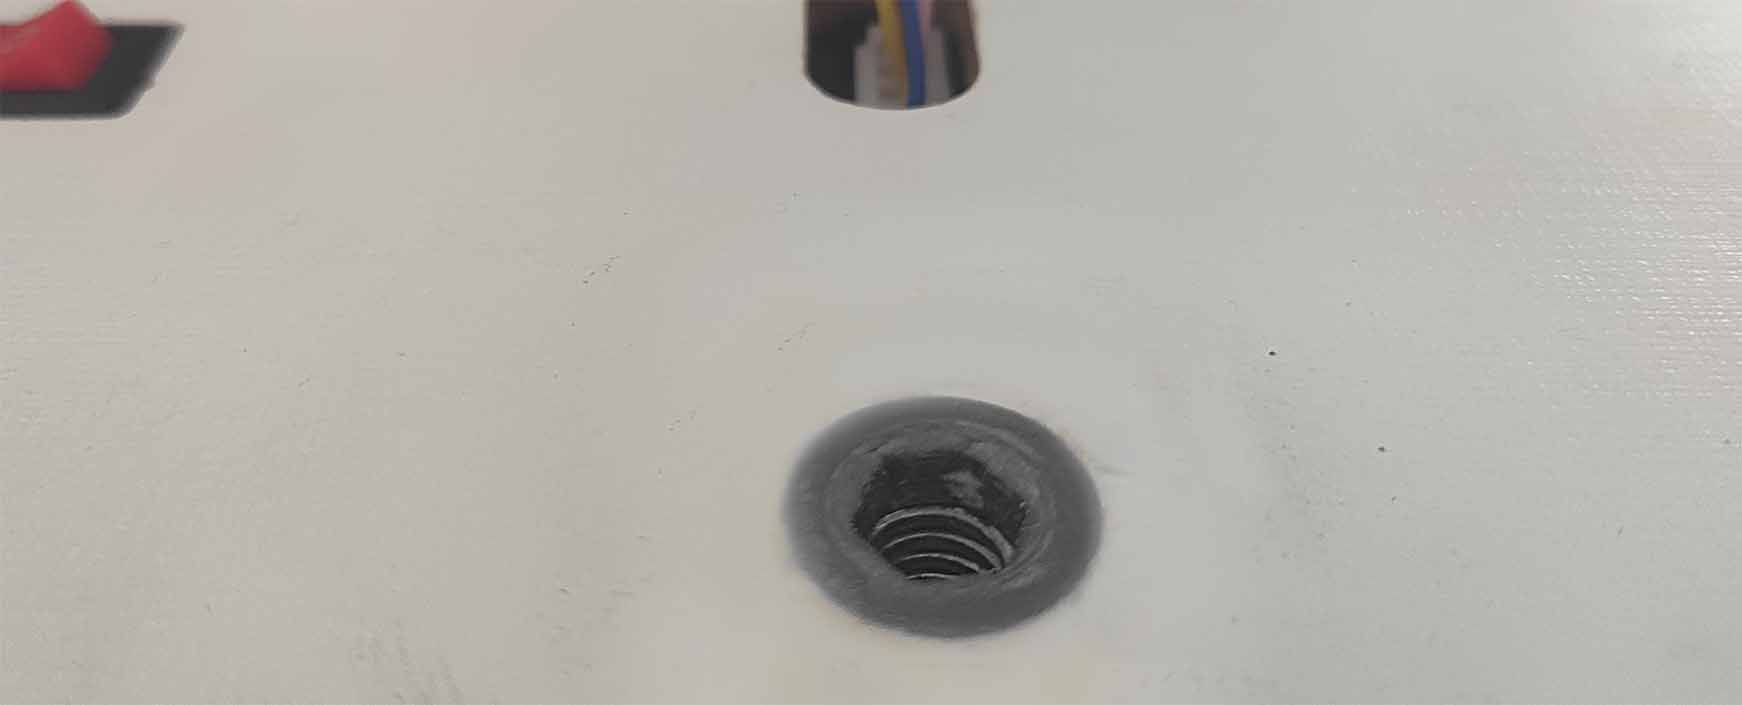
\includegraphics[width=\textwidth]{figuras/desPlataforma/insertoMontagem}
		\caption{}
		\label{fig:insertoMontagem}
	\end{subfigure}
	
	\fonte{Autor.}
\end{figure}

\begin{figure}[!htb]
	\centering
	\caption{Montagem da câmera no Ball Head}
	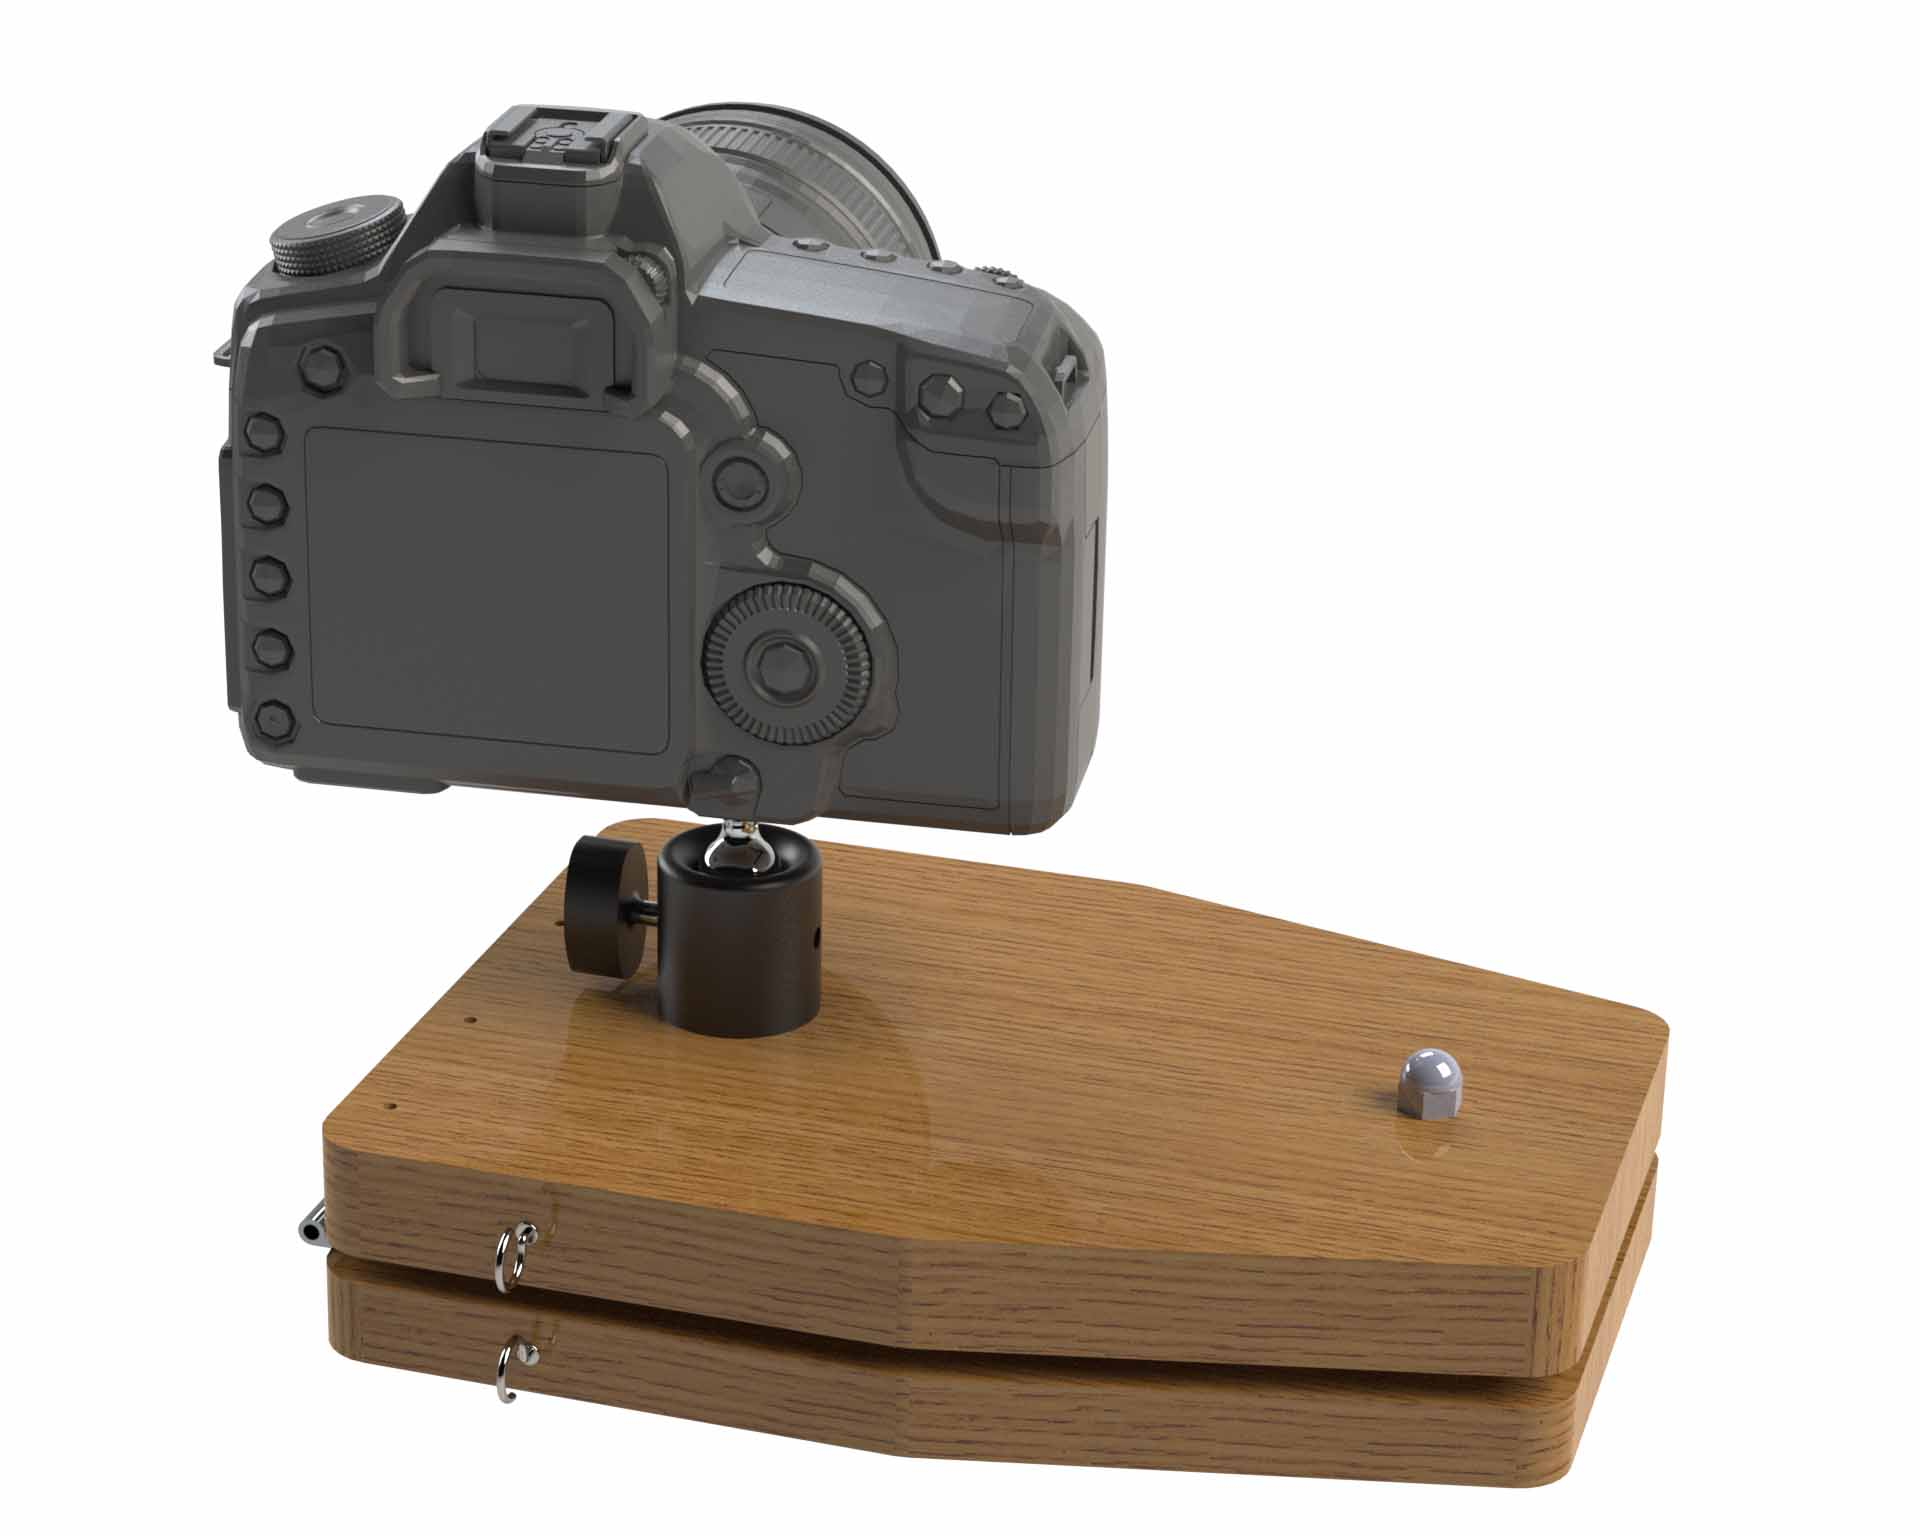
\includegraphics[width=.6\linewidth]{figuras/desPlataforma/montagemCamera}
	\label{fig:renderMontagemCamera}
	\fonte{Autor.}
\end{figure}

A estrutura e os componentes foram posicionados de forma que o projeto fosse compacto. O motor de passo é fixado na base inferior, e conecta-se em seu eixo uma engrenagem que irá transmitir o torque para movimentar a plataforma. O sistema de transmissão foi projetado para funcionar com duas engrenagens, que buscam suavizar o movimento do motor, reduzindo sua velocidade e aumentando o torque. A relação adotada no projeto foi 2:5\footnote{Cabe a observação de que a seleção de um padrão de uma relação de 2:5 nas engrenagens se motivou durante a realização dos cálculos a serem explicados a seguir, para que o motor trabalhe em uma velocidade e torque adequados. }, onde a engrenagem menor é montada no motor, e a maior transmite momento para o eixo curvado. A Figura \ref{fig:transmissao} demonstra a montagem da transmissão, com uma vista de corte na engrenagem menor e base da plataforma; a engrenagem menor está em verde, e a maior está em vermelho.

\begin{figure}[!htb]
	\centering
	\caption{Render que demonstra a transmissão do torque do motor para elevar a plataforma}
	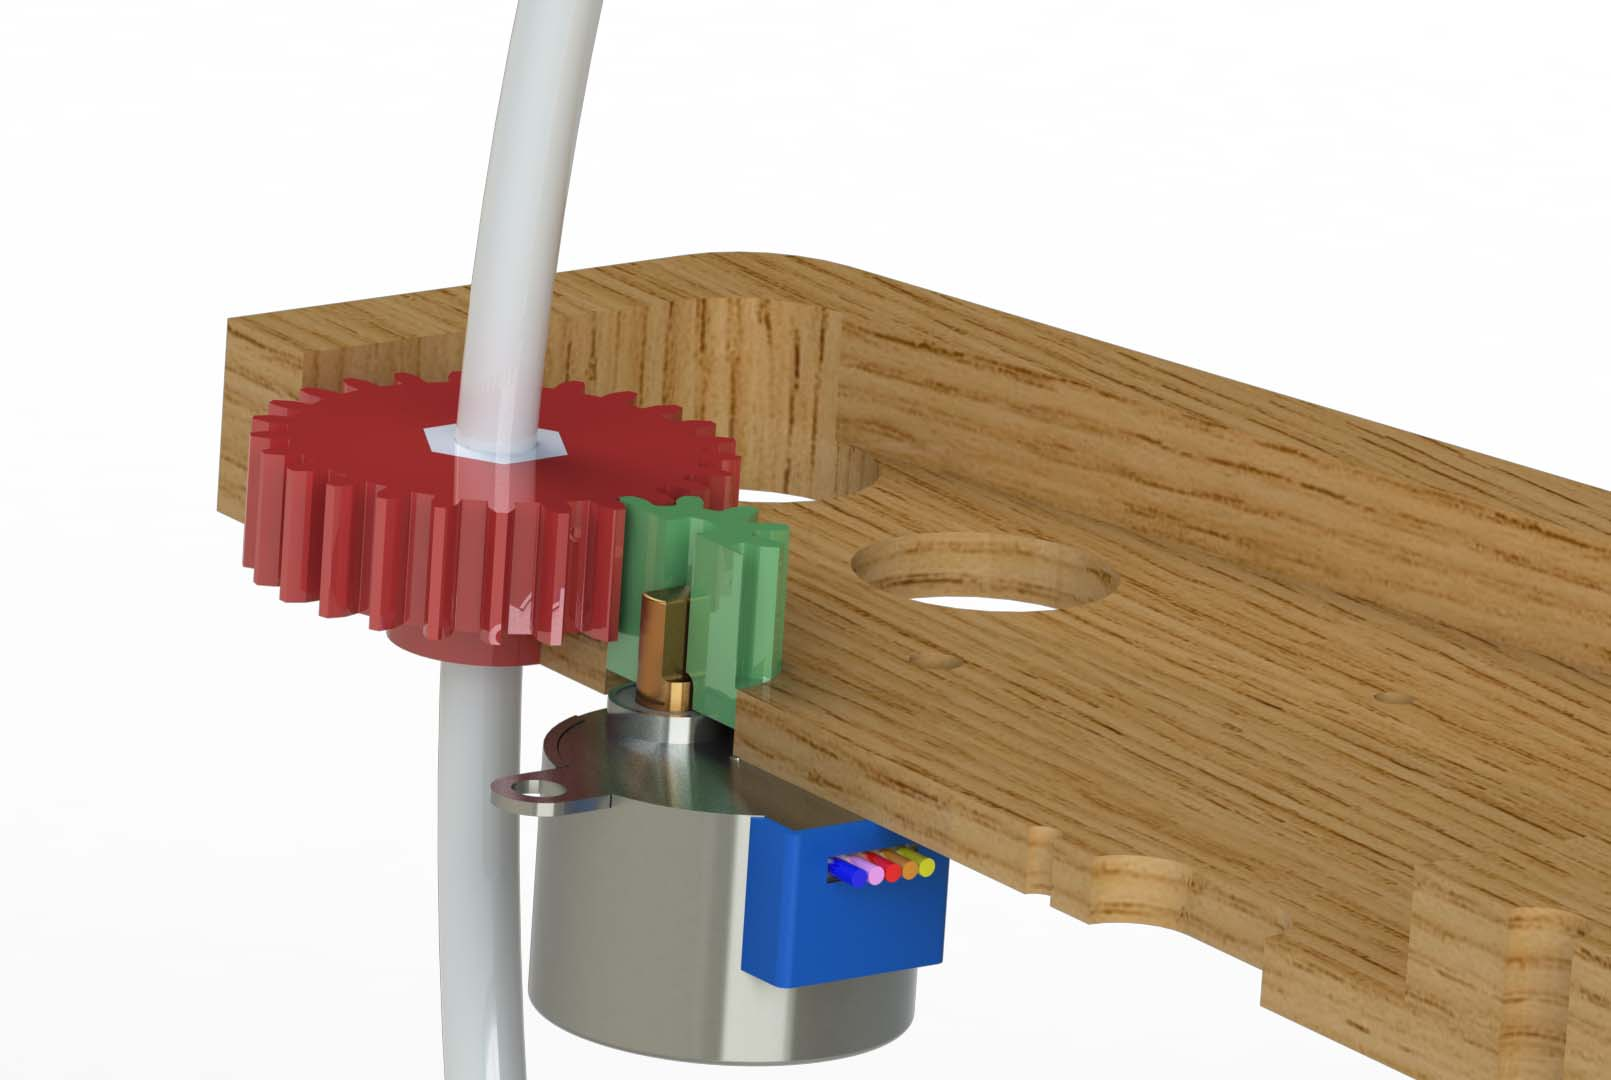
\includegraphics[width=.8\linewidth]{figuras/desPlataforma/transmissao}
	\label{fig:transmissao}
	\fonte{Autor.}
\end{figure}

Com base nas dimensões extraídas dessa montagem, foi avaliado matematicamente se o motor possuirá o torque necessário para rotacionar o sistema de transmissão. Para isso, se considera o cenário onde a câmera emprega maior força contra a plataforma, que é com o sistema totalmente fechado, com a base superior nivelada. As dimensões e variáveis usadas constam na Figura \ref{fig:calcDimens}. O Torque exercido no eixo curvo, pela câmera e equipamentos, é dado na equação (\ref{eq:torqueMontagem}), considerando: massa da câmera somada aos suportes e ball head $ m = 2,5~kg $; aceleração da gravidade $ g = 9,81~m/s^2 $; distância $ d_{ce} = 51~mm $ entre câmera e eixo de rotação da plataforma. 

\begin{figure}[!htb]
	\centering
	\caption{Representação da montagem com as dimensões para cálculos}
	\includegraphics[width=\linewidth]{figuras/desPlataforma/calcDimens}
	\label{fig:calcDimens}
	\fonte{Autor.}
\end{figure}

\begin{equation}
	\tau_{c} = m~g~d_{ce} = 1,370~Nm
	\label{eq:torqueMontagem}
\end{equation}

Dessa forma, a força $ F_{barra} $ que a barra roscada deve exercer para mover a câmera é dada na equação (\ref{eq:forcaBarra}). Considerando, também,  que a distância $ d_{eb} $entre o eixo e a barra roscada é de $ 179~mm $.

\begin{equation}
	F_{barra} = \dfrac{\tau_{c}}{d_{eb}}= 7,6~N
	\label{eq:forcaBarra}
\end{equation}

Então, o torque empregado na engrenagem maior, que está em contato com a barra rosqueada é dado na equação (\ref{eq:torqueEng}) \cite{}. Essa equação considera o passo da rosca na barra roscada $ p = 1~mm $; e uma eficiência de rotação $ e $ igual a $ 0,15 $ \cite{man:pcblinear}. Esse último fator nasce pelo atrito na transmissão em uma rosca sem lubrificação, e ele pode sofrer alterações de acordo com o fabricante. Como esse valor é incerto e depende da montagem; e além disso, não existe um padrão na eficiência, e por isso considerou-se o menor valor obtido em catálogos de fabricantes. 

\begin{equation}
	\tau_{eng2} = \dfrac{F_{barra}\times p\div (2\pi)}{e} = \dfrac{9,2 \times 0,00159}{0,1} = 8,134 mN.m 
	\label{eq:torqueEng}
\end{equation}

Após isso, considerando a relação de 2:5 adotada entre as duas engrenagens, calcula-se o torque máximo do motor, $ \tau_{max} $, com a equação (\ref{eq:torquemotor}). Além disso, se adiciona um coeficiente de segurança para o torque de um motor de passo que é igual à 1,5 \cite{man:sizemotor}. Dessa forma, têm-se um torque máximo necessário igual a $ 5,85~mN.m $, que respeita o limite de 34,3~mN.m


\begin{equation}
	\tau_{max} = \tau_{eng1} = \tau_{eng2} \times 2 \div 5 \times 1,5 = 5,85 ~mN.m
	\label{eq:torquemotor}
\end{equation}


A velocidade do motor também foi calculada com a equação \ref{eq:speed}. Ela considera que a rotação completa da câmera, com a plataforma, seria de $ 23~h $ e $ 56~min $; o raio de rotação do sistema ($ r_{sis} $)  é de $ 179~mm $, medindo do eixo da dobradiça até a barra curvada; o passo da barra roscada M6 que é de $ 1~mm $; e a relação entre as engrenagens, de 2:5. O valor calculado de $ 1,96~rpm $ é adequado pois respeita a relação de Torque máximo \textit{versus} Velocidade do Motor\footnote{Essa curva de torque pela velocidade não existe oficialmente. Em muitos fóruns essas curvas são discutidas e medidas experimentalmente. Neste link consta uma das curvas extraídas e que demonstram a aplicabilidade dessa relação de torque e velocidade adotadas, considerando que $ 2~rpm $ implicam em $ 143 $ \textit{half-steps} por segundo: \url{https://forum.arduino.cc/t/28byj-48-5v-stepper-100-rpm/575338}} 

\begin{equation}
	V(rpm) = \dfrac{2\times\pi\times0,179\div0,001}{23\times60+56}\times\dfrac{5}{2} = 1,96~rpm
	\label{eq:speed}
\end{equation}



\subsection{Engrenagens}

Tendo em vista a confirmação do dimensionamento dado anteriormente, foi realizado o projeto das engrenagens. Devido à customização do projeto, optou-se por fabrica-las com impressão 3D. Dentro disso, considerando os materiais mais comuns utilizados nas impressoras (PLA, ABS e PETG), optou-se pelo PLA em função de sua resistência mecânica e baixo custo \cite{site:3dprinted}. 

Para a modelagem, foi calculado as dimensões de projeto para engrenagens de dente retos, que são adequadas para prototipagem com impressão 3D. Essas dimensões tem como base o diâmetro externo de uma das engrenagens; o Ângulo de pressão, que é igual para ambas; e o número de dentes \cite{site:3dprinted}.  


O ângulo de pressão adotado é o padrão de mercado: $ \theta = 20^{\circ} $; e o diâmetro externo ($ d_e $) da engrenagem menor foi definido tendo como base o espaço máximo que poderia ocupar na plataforma, que é de $ 16~mm $. Definiu-se também que a engrenagem maior terá 10 dentes ($ Z $), e consequentemente, pela relação 2:5, a maior terá 25 dentes.


Além disso, módulo da engrenagem é um valor que deve ser igual em ambas, e é utilizado como parâmetro para o cálculo das demais medidas de projeto. Com a equação (\ref{eq:modulo},) calculou-se $ m = 1,33 $ . Com ele, define-se também que a espessura mínima das engrenagens é de  $ b = 8~mm $; ela é calculada pela equação (\ref{eq:espMinima}). Dessa forma, para o projeto, foi determinado que a espessura seria de $ b = 10~mm $, encaixando na profundidade do rasgo feito na base inferior da plataforma. Assim, a tabela \ref{tab:engrenagens} sintetiza os demais valores calculados, que estão exemplificados na Figura \ref{fig:engProj} \cite{tcc:lucasEngrenagem}.

\begin{equation}
	m = \dfrac{de}{Z+2}
	\label{eq:eq:modulo}
\end{equation}

\begin{equation}
	b > 6 \times m
	\label{eq:eq:espMinima}
\end{equation}

\begin{figure}[htb]
	\centering
	\caption{Dimensões de projeto para engrenagens}
	\includegraphics[width=\linewidth]{figuras/desPlataforma/engProj}
	\label{fig:engProj}
	\fonte{Adaptado de \cite{tcc:lucasEngrenagem}.}
\end{figure}

\begin{table}[!htb]
	\centering
	\caption{Cálculos das dimensões para engrenagens}
	\begin{tabular}{r|c|c|c}
		Medida & Eng. menor (mm) & Eng. maior (mm) & equação\\
		Diâmetro Externo ($ de $) & 16,00 & 36,02 & (\ref{eq:de})\\
		Diâmetro Primitivo ($ dp $) & 13,33 & 33,35 & (\ref{eq:dp})\\
		Diâmetro de Base ($ db $) & 12,53 & 31,34 & (\ref{eq:db})\\
		Diâmetro Interno ($ di $) & 10,45 & 30,46 & (\ref{eq:di})\\
		Passo ($ P $) & 4,19 & 4,19 & (\ref{eq:passo})\\
		Espessura do Dente ($ ed $) & 2,09 & 2,09 & (\ref{eq:vao})\\
		Vão ($ v $) & 2,09 & 2,09 & (\ref{eq:vao})\\
		Filete ($ f $) & 0,22 & 0,22 & (\ref{eq:f})\\
	\end{tabular}
	\label{tab:engrenagens}
\fonte{Autor.}
	
\end{table}

\begin{equation}
	de = m \times (Z + 2)
	\label{eq:de}
\end{equation}

\begin{equation}
	dp = m \times Z
	\label{eq:dp}
\end{equation}

\begin{equation}
	db = dp\times\cos \theta
	\label{eq:db}
\end{equation}

\begin{equation}
	di = de-(2,166\times m)
	\label{eq:di}
\end{equation}

\begin{equation}
	P = m\pi
	\label{eq:passo}
\end{equation}

\begin{equation}
	v = ed = \dfrac{P}{2}
	\label{eq:vao}
\end{equation}

\begin{equation}
	f = \dfrac{m}{6}
	\label{eq:f}
\end{equation}


\subsection{Barra de Elevação}

A barra de elevação curva é o componente que realiza a elevação da base superior, recebendo o movimento da engrenagem maior através de uma porca sem travante, fixada na engrenagem. A porca é inserida na engrenagem, como ilustra a Figura \ref{fig:explosao}, e se mantêm por meio de um colante \textit{TeekBond}. 

\begin{figure}[htb]
	\centering
	\caption{Vista Explodida da engrenagem maior com a porca e a barra rosqueada}
	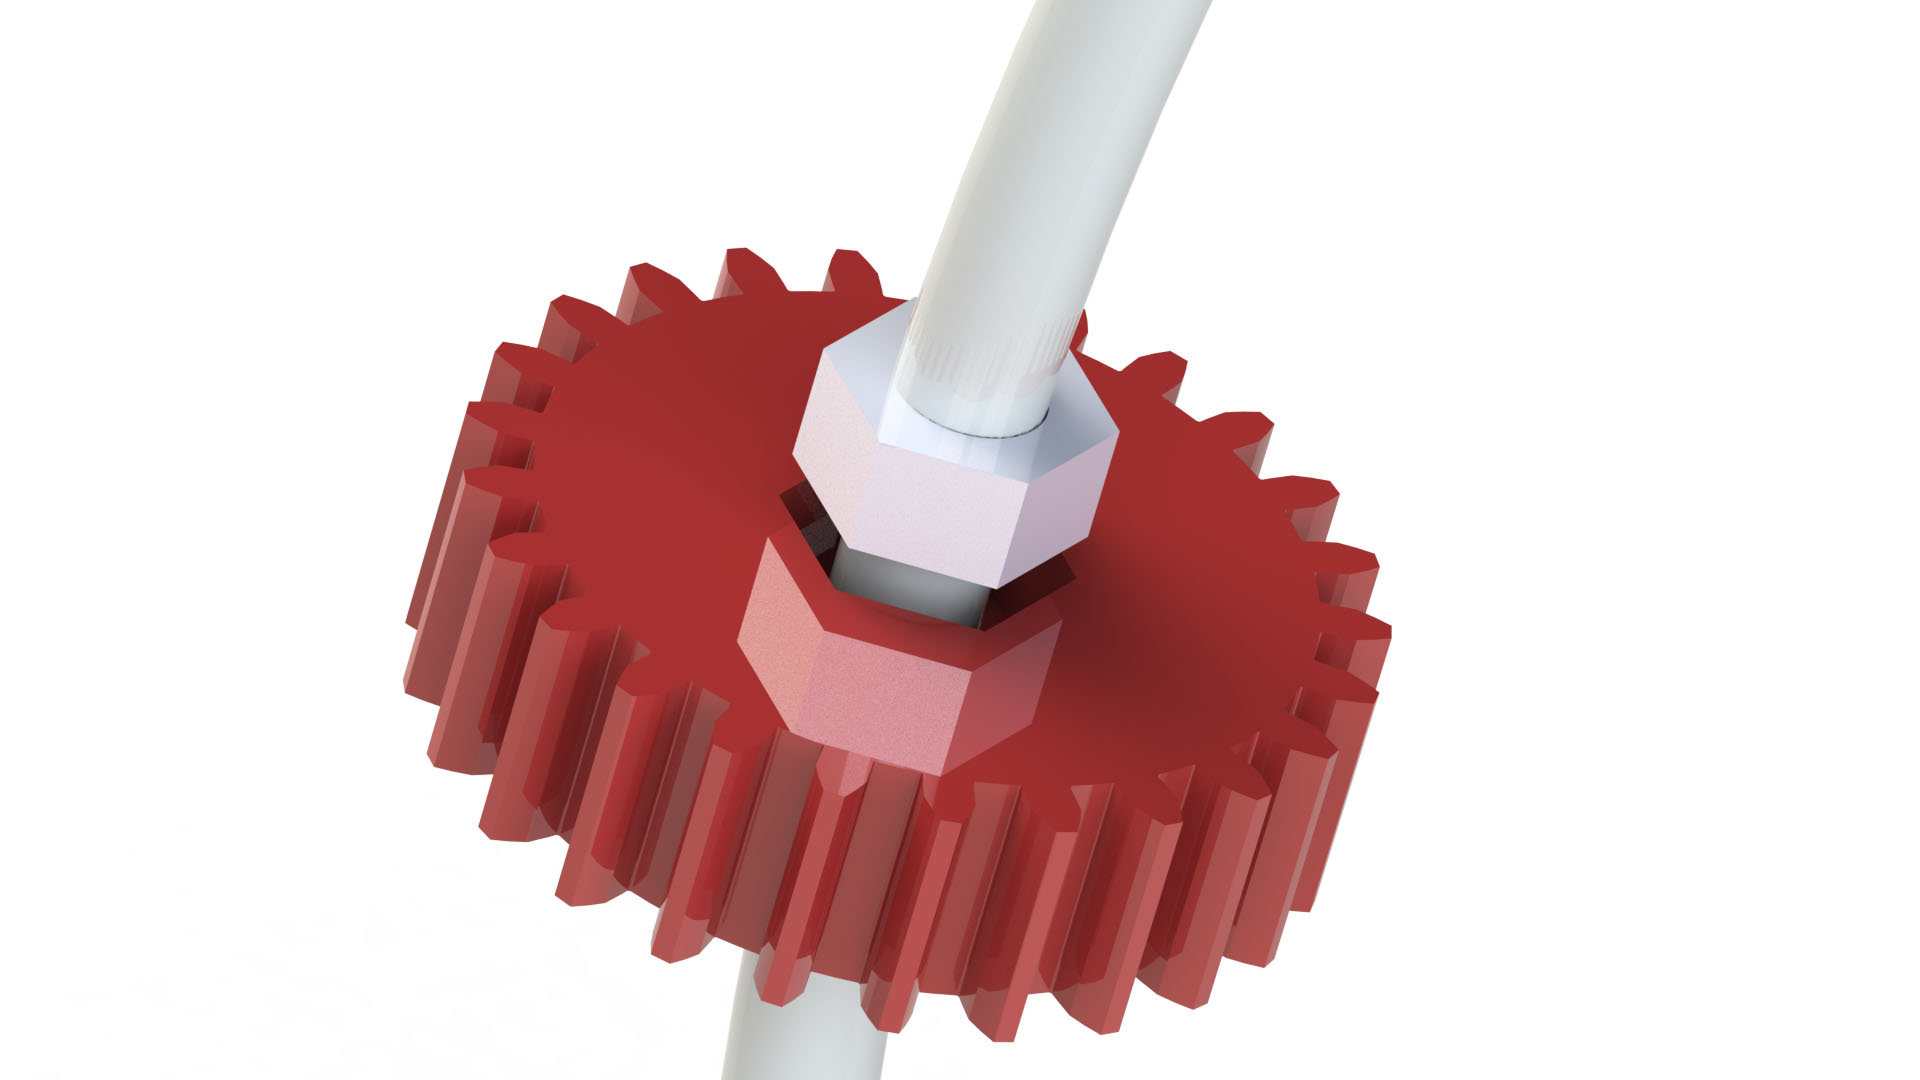
\includegraphics[width=0.6\linewidth]{figuras/desPlataforma/explosao}
	\label{fig:explosao}
	\fonte{Autor.}
\end{figure}

Essa barra é comercializável somente em formato reto, sem curvatura. O processo de dobra pode ser feito de forma artesanal ou com equipamentos especializados. Para o projeto, fez-se a dobra de forma manual, corrigindo imperfeições até que o resultado ficasse o mais próximo possível do projetado. Essa conferência é realizada com o gabarito no apêndice \ref{apendice:barracurvada}. 


Por isso, destaca-se que barra de elevação pode se tornar o principal causador de problemas na estabilidade do sistema, pois é curva. A curvatura pode gerar instabilidade no contato com a engrenagem e, se não for fabricada de maneira precisa, pode criar certas incertezas no funcionamento. 

\subsection{Placa de Circuíto}
Para finalizar o projeto mecânico, foi inserido um modelo 3D do circuito impresso, garantindo que os componentes mecânicos e eletrônicos estão projetados corretamente, alinhando furos de fixação e de botões. A Figura \ref{fig:renderEasyTracker} renderiza como ficou o projeto final.

\begin{figure}[!htb]
	\centering
	\caption{Render do projeto final}
	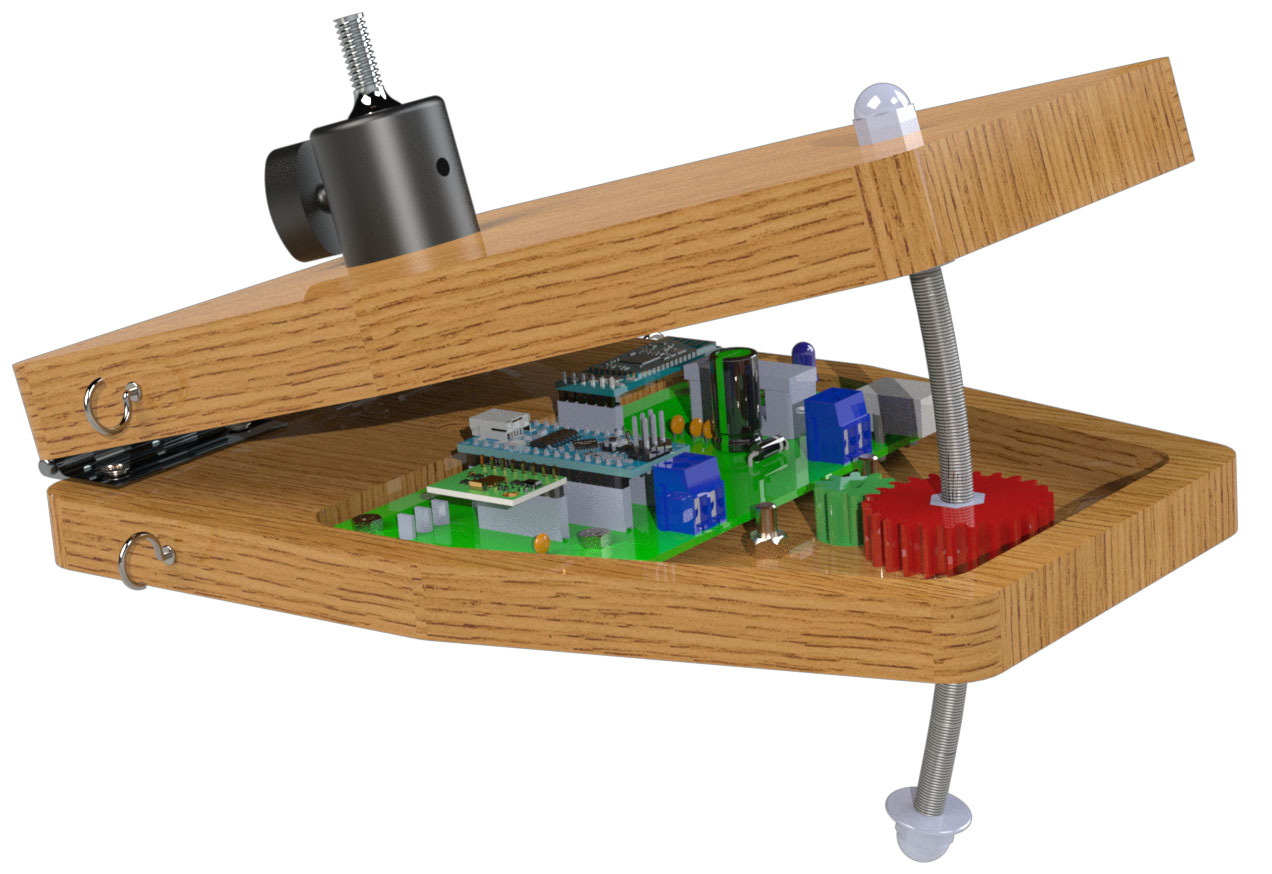
\includegraphics[width=.95\linewidth]{figuras/desPlataforma/renderEasyTracker}
	\label{fig:renderEasyTracker}
	\fonte{Autor.}
\end{figure}

\section{Montagem}

Todos os componentes foram Fabricados e Montados, e o resultado pode ser acompanhado na Figura \ref{fig:montagemReal}. Nela, é possível reparar alguns detalhes como o Ball Head Maxxi Grua utilizado para fixar a câmera na base superior. Além disso, foi inserido na montagem física um conjunto de 4 elásticos que colaboram para amortecer a vibração do sistema, que será detalhada na Seção \ref{sec:vibracao}.

%\begin{enumerate}
%	\item Rosca 1/4" na base inferior usando a Chave Allen xx
%	\item Parafusos de Fixação da PCB na base inferior
%	\item Placa de circuíto é posicionada nos parafusos, onde é fixada.
%	\item Dobradiças conectando base superior e inferior
%	\item Motor de Passo com engrenagem menor é parafusado na base inferior
%	\item Ball-Head da câmera é parafusado na base superior
%	\item Engrenagem maior rosqueada no eixo curvo
%	\item Eixo curvo é fixado na base superior com 2 porcas, 2 arruelas e 2 borrachas (uma em cada lado da base).
%	\item Rosqueiam-se os ganchos e instalam-se os elásticos.
%\end{enumerate}

%Então, com base em todos os documentos e arquivos de projeto, fabricou-se os componentes e a plataforma equatorial foi montada. Na Figura \ref{fig:montagemReal} é possível ver a montagem pela vista lateral esquerda.


\begin{figure}[!htb]
	\centering
	\caption{Vista lateral da montagem final do sistema}
	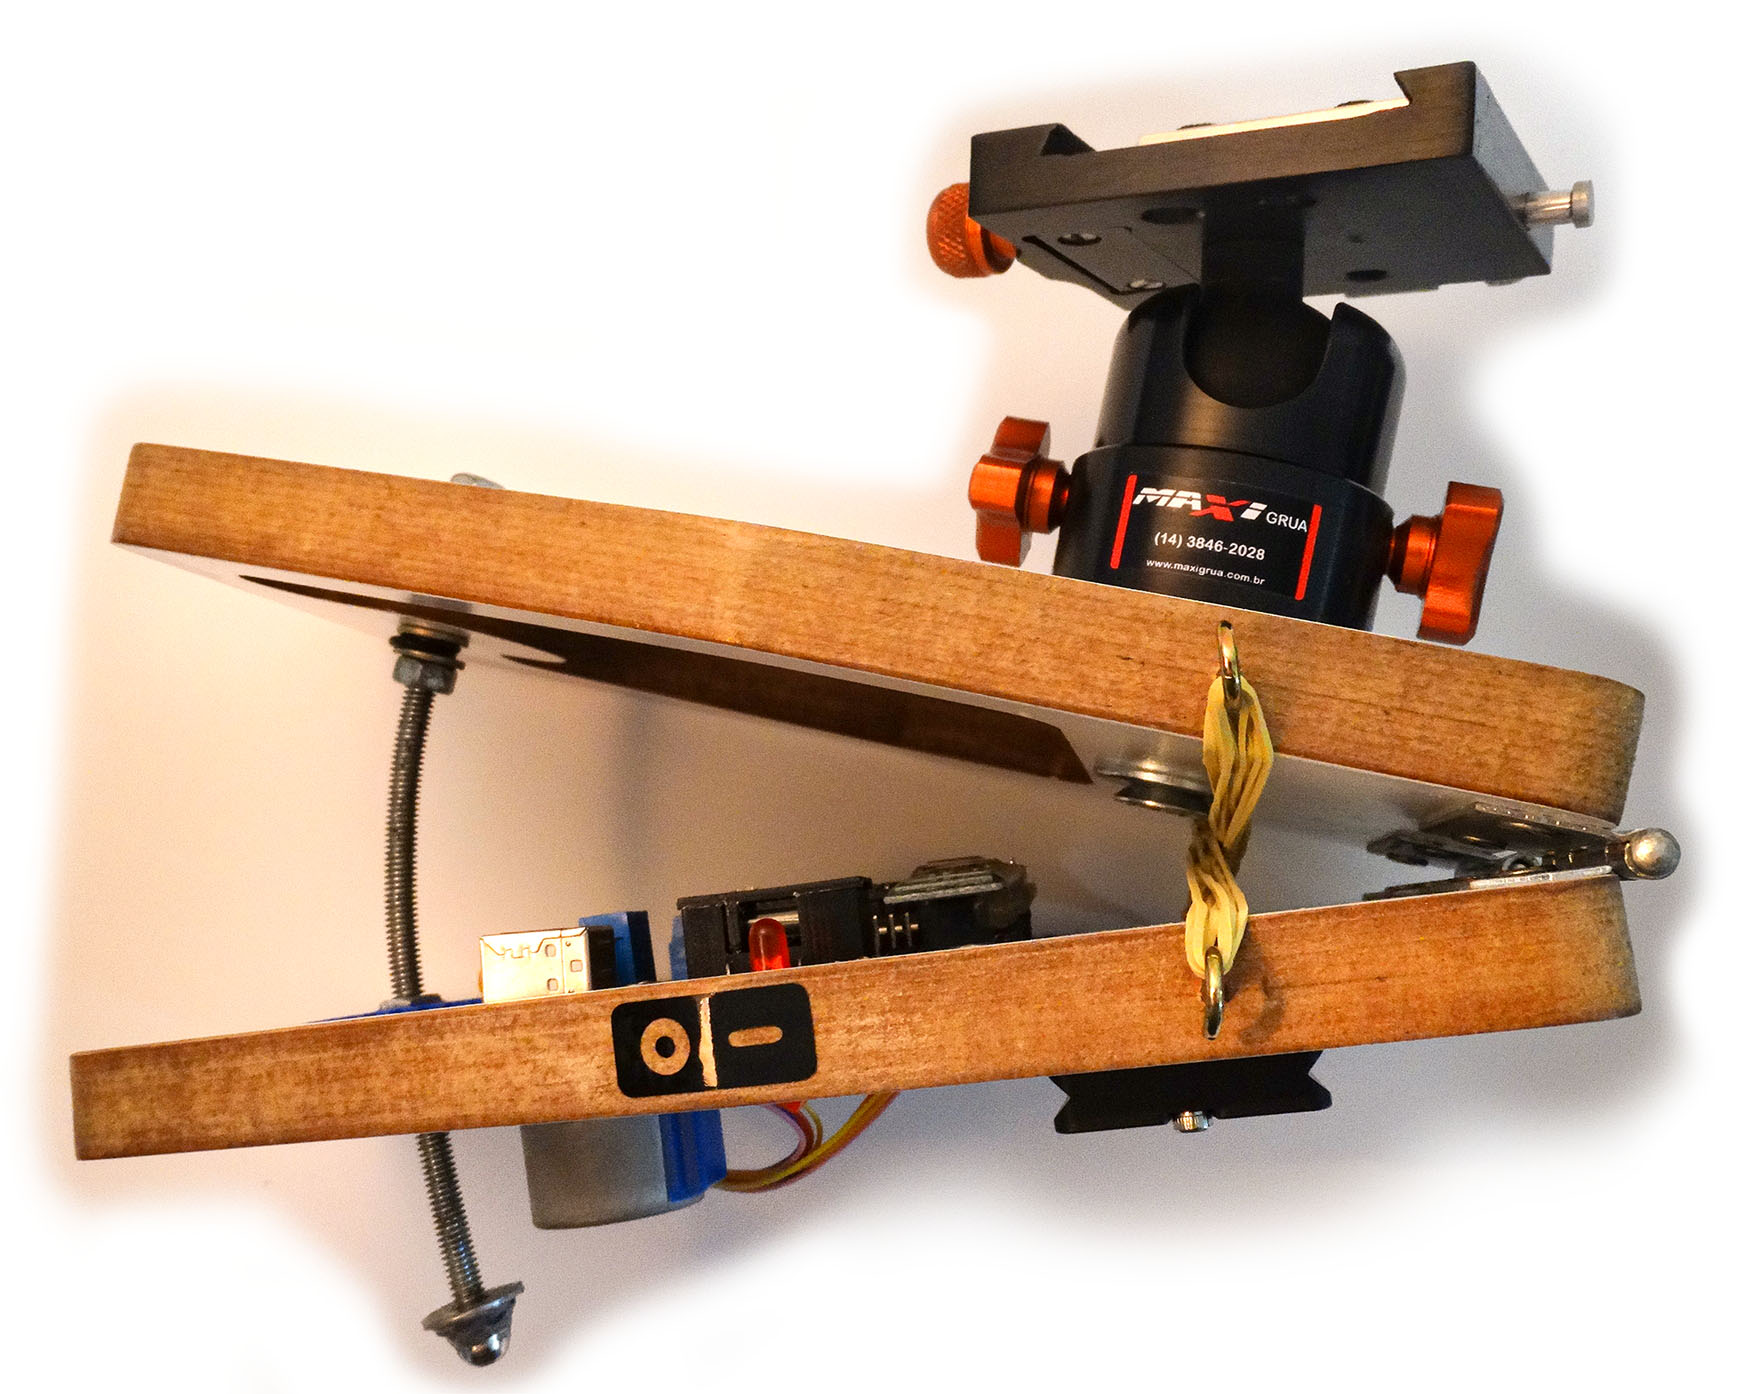
\includegraphics[width=.8\linewidth]{figuras/desPlataforma/montagemReal}
	\label{fig:montagemReal}
	\fonte{Autor.}
\end{figure}

\section{Hardware Eletrônico}

O Hardware que foi apresentado em CAD na última subseção embarca o Arduíno, Driver do Motor de passo, botões de controle, além dos módulos Bluetooth e de sensores. 

\subsection{Arduíno Nano}
Para realizar o controle do sistema, foi empregado o controlador ATMEGA328P com um Arduíno Nano (Figura \ref{fig:pinoutNano}). Esse controlador tem somente um núcleo de processamento de 16MHz, além de pinos de comunicação I2C, UART, entre outros \cite{man:pinoutNano}. Ele foi escolhido por ter uma ampla documentação na internet, uma variedade de bibliotecas, e ser um dos mais acessíveis do mercado, principalmente no Brasil. 

\begin{figure}[htb]
	\centering
	\caption{Pinagem do Arduíno Nano}
	\includegraphics[width=\linewidth]{figuras/desPlataforma/pinoutNano}
	\label{fig:pinoutNano}
	\fonte{Adaptado de \cite{man:pinoutNano}.}
\end{figure}

\subsection{Módulo Bluetooth HC05}
Para a comunicação Bluetooth, foi escolhido o Módulo HC05, que utiliza protocolo Serial UART de comunicação e consequentemente é compatível com o controlador ATMEGA328P. O Módulo, mostrado na Figura \ref{fig:hc05}, possui os 2 pinos RX e TX de comunicação, VCC e GND de alimentação, e ainda outros 2 pinos: STATE e KEY/EN. O pino STATE indica que o módulo está pareado com algum outro dispositivo. O segundo é utilizado para permitir que o controlador altere parâmetros internos do sistema Bluetooth \cite{}. O módulo embarca o chip HC05, LEDs indicadores, além de componentes passivos de alimentação e funcionamento da rede UART.

 %todo citação e imagem hc05
\begin{figure}[!htb]
	\centering
	\caption{Módulo HC05 e suas conexões.}
	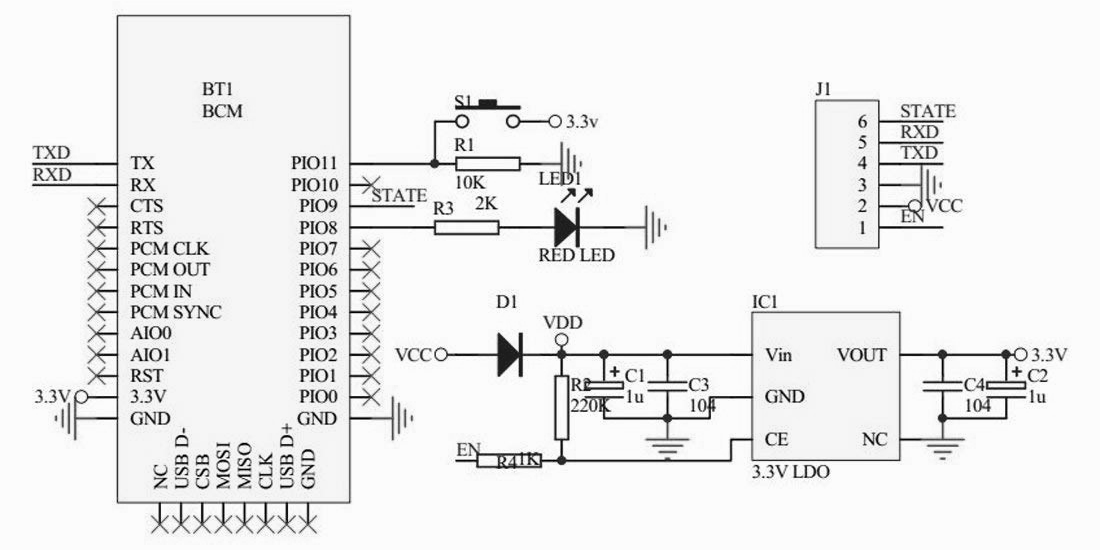
\includegraphics[width=\linewidth]{figuras/desPlataforma/HC05}
	\label{fig:hc05}
	\fonte{Adaptado de \cite{}.}
\end{figure}

\subsection{Módulo de sensores GY87}
O sensoreamento da plataforma, para guiar o alinhamento equatorial, é realizado pelo conjunto de sensores MPU6050 -- acelerômetro e giroscópio -- e HMC5883 -- magnetômetro --, pois ambos podem ser conectados facilmente em um Arduíno usando um módulo GY87. A conexão é realizada com rede I2C, no entanto, existem ressalvas quanto ao circuito do módulo, mostrado na Figura \ref{fig:gy87}.

É possível reparar na Figura que a rede I2C do módulo conecta somente com as conexões do MPU6050 (H\_CL e H\_DA), e no módulo HMC5883 essa comunicação ocorre com os pinos I2C auxiliares do MPU6050 (AUX\_DA e AUX\_CL). Então, para que o HMC seja conectado diretamente com a rede I2C do módulo, é preciso configurar o MPU para que ele internamente interconecte os pinos H\_CL com AUX\_CL e H\_DA com AUX\_DA.  Essa configuração é realizada no registrador 55 do MPU6050, setando-o em 1 \cite{man:mpu6050}. Além disso módulo já conta com os resistores da rede I2C e os capacitores de filtro de alimentação do circuíto.

\begin{figure}[!htb]
	\centering
	\caption{Diagrama Esquemático do Módulo}
	\includegraphics[width=0.9\linewidth]{figuras/desPlataforma/gy87}
	\label{fig:gy87}
	\fonte{Adaptado de \cite{man:gy87}.}
\end{figure}

\subsection{\textit{Driver} ULN2003}
Para controle do Motor de Passo foi escolhido o \textit{driver} ULN2003, que normalmente é comprado junto com o motor. Com ele, é possível realizar controle \textit{Full} e \textit{Half step}, operando com 5V e sendo compatível com um Arduíno. O \textit{driver} consegue controlar até 8 bobinas, e por isso só 4 portas de entrada e saída serão ocupadas. Esse \textit{driver} é composto por um \textit{array} de 8 transistores \textit{Darlington} onde o comando de cada transistor é enviado por um pino do controlador, e a saída do transistor é conectada em uma fase do motor . Dessa forma, o driver consegue prover corrente necessária para o funcionamento adequado do rotor\cite{man:ulndriver}.

\subsection{Alimentação do Sistema}
Optou-se por realizar a alimentação do sistema eletrônico com \textit{powerbanks} de 5V, com um circuito de proteção entre o \textit{powerbank} e os demais componentes. Esses circuito utiliza um fusível e um diodo zenner. O fusível tem a função de impedir um surto de corrente: quando há um curto no sistema, por exemplo, o fusível arrebenta, interrompendo a passagem de energia. Do contrário, o diodo Zenner 1N5338BRL, que foi selecionado, trabalha com uma faixa de tensão de 5.1V; quando a tensão se elevar acima desse ponto de operação, o diodo entrará em condução, impedindo que os componentes da placa queimem pelo aumento de tensão \cite{man:diodozenner}. 

Fazer com que a alimentação do sistema seja de 5V torna ela compatível com as portas USB de celulares. Dessa forma, se o equipamento é utilizado longe de qualquer fonte de energia elétrica, é possível mantê-lo funcionando somente com um celular e um cabo de alimentação. 

\subsection{Diagrama Elétrico}

Todos esses fatores combinaram para a criação do esquemático da PCB que está na Figura \ref{fig:BDT_TCC_rev4}. 
\begin{figure}[!htb]
	\centering
	\caption{Diagrama elétrico final}
	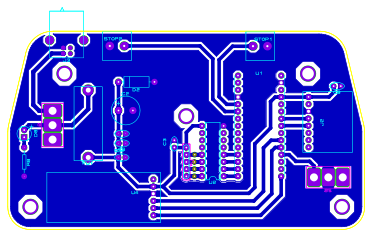
\includegraphics[width=\linewidth]{figuras/desPlataforma/BDT_TCC_rev4}
	\label{fig:BDT_TCC_rev4}
	\fonte{Autor.}
\end{figure}




\subsection{\textit{Layout}}
O layout foi desenvolvido utilizando o espaço reservado na base inferior e nos locais de fixação, respeitando as limitações dos protocolos de comunicação e recomendações de desenvolvimento para os componentes. São cinco pontos de fixação, dos quais quatro localizam-se em cada canto, e o quinto foi instalado no centro, onde planejou-se deixar o conector do motor de passo. O conector USB do tipo B e botões de controle foram posicionados próximos dos cantos da placa. Esses posicionamentos garantem que a placa não irá fletir quando o usuário estiver montando-a ou realizando um acionamento. 

Além desse fator, os componentes foram organizados para serem agrupados em 4 zonas: Alimentação, Dados, Controle e Comunicação \textit{Bluetooth} (Figura \ref{fig:zonasPcb}). Buscou-se manter a zona de dados o mais distante possível do sistema \textit{Bluetooth}, e o mais próximo possível do Arduíno, para reduzir a impedância das linhas SDA e SCL do protocolo I2C dos sensores.

\begin{figure}[!htb]
	\centering
	\caption{Regiões da PCB}
	\includegraphics[width=0.7\linewidth]{figuras/desPlataforma/zonasPCB}
	\label{fig:zonasPcb}
	\fonte{Autores.}
\end{figure}  

Foi criado um plano de Terra apenas na parte inferior da placa, onde os componentes são soldados. Assim, a placa pode ser fabricada em modos mais simples e artesanais. Por isso, também, manteve-se uma distância de $ 0,75 cm $ entre trilhas, e dos componentes com o plano de terra; visto que distâncias menores podem incorrer em curtos durante o processo de fabricação. A figura \ref{fig:pcbBot} mostra o projeto da PCI.

\begin{figure}[!htb]
	\centering
	\caption{Projeto da Placa de Circuito Impresso}
	\includegraphics[width=0.7\linewidth]{figuras/desPlataforma/pcbBot}
	\label{fig:pcbBot}
	\fonte{Autor.}
\end{figure}


\subsection{Fabricação do Circuíto}
A placa foi fabricada com CNC e os componentes, todos PTH(Pin Through Hole), foram soldados com ferro de solda. Após esses processos, foi aplicado um verniz isolante de PCI -- Isotec \textregistered ~-- da Implastec, para protegê-la contra umidade, visto que a plataforma será usada em ambientes noturnos, ficando exposta ao orvalho e sereno.

\section{Software Embarcado}

As instruções do ATMEGA328p foram desenvolvidas em C++ na IDE do Arduíno, e são o software que irá embarcar o microcontrolador\footnote{O código está disponível no Github neste link: LINK AQUI}. Foram utilizadas bibliotecas adquiridas no GitHub\footnote{As licenças para uso dessas bibliotecas foram respeitadas em conjunto com o licenciamento do projeto} para os sensores, comunicação e controle do motor. Elas foram adaptadas e organizadas para simplificar o código, tornando-o mais eficiente. 

A eletrônica tem como principais funções realizar o controle do motor; ler e processar os dados dos sensores inerciais, enviando os dados dos ângulos calculados para o aplicativo \footnote{As informações sobre o processamento e protocolo de comunicação implementados estão na seção \ref{sec:btandroid}}. Além disso, deve processar o controle dos botões pelo usuário, tanto os botões físicos, como os botões virtuais do aplicativo, cuja alternância de estado é processada na comunicação bluetooth. 

O processamento dos dados dos sensores inerciais foi implementado com os algoritmos descritos na seção \ref{sec:calcPitchRoll}, para o cálculo de Pitch e Roll; e seção \ref{sec:azimutal} para algoritmo de cálculo do ângulo azimutal com o magnetômetro. As informações de calibração do magnetômetro foram armazenadas na EEPROM do ATMEGA328P, onde foram utlizados 12 dos 1024 bytes disponíveis \cite{man:atmegadatasheet}.

O módulo de sensores usa comunicação I2C, enquanto o módulo Bluetooth utiliza comunicação UART. O código que implementa a comunicação com esses módulos está descrito nas bibliotecas, respectivamente. O algoritmo dessas bibliotecas está adequado em consoância com o descrito nas seções \ref{sec:uart} e \ref{sec:i2c}.
